\chapter{Statistical distributions}
\begin{refsection}

\abstract{This unit calculates the most important distributions and their integrals. The routines are based on \parencite{Abr-64,Noa-80,Kin-82,Pre-89,PCSig-94}. All probabilities are given in mathematical form, that is in the rage of \(0\ldots 1 \).}

The unit has the following interface:
\begin{lstlisting}[caption=Interface of \texttt{Stat}]
  UNIT Stat;

  INTERFACE

  USES Math, mathfunc;

  CONST
    StatError: BOOLEAN = FALSE;   // toggle FOR error condition

  { **************************** F-distribution **************************** }

  FUNCTION Integral_F(F: float; f1, f2: LONGINT): float;

  FUNCTION Finv( Alpha, Dfn, Dfe: float ) : float;

  { ************************** t-distribution ****************************** }

  FUNCTION Integral_t(t: float; f: LONGINT): float;

  FUNCTION SignificanceLimit_t(p: float; f: LONGINT): float;

  PROCEDURE CompareLiterature(VAR t: float; Average, Sta, Literatur: float;
                              VAR f: LONGINT; n: LONGINT);

  PROCEDURE UnequalSigma(VAR t: float; Average1, Average2, sta1, sta2: float;
                         VAR f: LONGINT; n1, n2: LONGINT);

   { ************************** X2-distribution **************************** }

  FUNCTION IntegralChi(ChiSqr: float; f: WORD): float;

  FUNCTION SignificanceLimit_Chi2 (p : float; dgf : WORD) : float;

  FUNCTION SigChi( Chisq , Df : float ) : float;

  { ***********************  normal distribution *************************** }

  FUNCTION IntegralGauss(z: float): float;

  FUNCTION SignificanceLimitGauss(WantedSecurity: float): float;

  FUNCTION NormalStandardValue (P : float) : float;

  FUNCTION Erf( Z : float ) : float;

  FUNCTION SigNorm (X : float) : float;

  FUNCTION NinvCoarse( P : float ) : float;

  FUNCTION Ninv( P : float ) : float;

  FUNCTION CDNorm (X : float) : float;

  { ********************** binomial distribution *************************** }

  FUNCTION BinominalFrequency (Trials, Success: LONGINT; P: float): float;

  FUNCTION BinominalIntegral (Trials, Value: LONGINT; P: float): float;

  { ************************ Pareto distribution *************************** }

  FUNCTION IntegralPareto (x, Minimum, Shape: float): float;

  FUNCTION PDFPareto (x, Minimum, Shape: float): float;

  { ************************* beta-distribution **************************** }

  FUNCTION CDBeta (X, Alpha, Beta : float; Dprec, MaxIter : INTEGER;
                   VAR Cprec : float; VAR Iter, Ifault : INTEGER  ) : float;

  FUNCTION BetaInv (P, Alpha, Beta : float; MaxIter, Dprec: INTEGER;
                    VAR Iter : INTEGER; VAR Cprec : float; VAR Ierr: INTEGER) : float;

  { ************************* gamma-distribution *************************** }

   FUNCTION ALGama ( Arg : float ) : float;

  FUNCTION GammaInt (Y, P : float; Dprec, MaxIter : INTEGER;
                     VAR Cprec : float; VAR Iter, Ifault  : INTEGER ) : float;

  FUNCTION KolmogorovSmirnovIntegral (alam: float): float;


  IMPLEMENTATION

  CONST Xln2sp   = 0.918938533204673;      // LogE(Sqrt(2 * CONST_PI))
        MaxPrec  = 16;                     // Max. precision
        LnTenInv = 1/Const_ln10;           // 1 / LN(10)

  var ch : char; // for error reporting
\end{lstlisting}

\section{F-distribution}

Integration of the \skalar{F}-distribution gives the probability for the 0-hypothesis that two series of measurements have the same standard deviations. Both series must be normally distributed and free of outliers.

\begin{lstlisting}[caption=Routines for the F-Distribution]
  FUNCTION Integral_F(F: float; f1, f2: LONGINT): float;

  VAR
    S, X, A, B, V: float;


    FUNCTION R0(M, N: LONGINT; V: float): float;

    VAR
      G, Sum: float;
      k, TEST: LONGINT;

    BEGIN
      k := 1;
      G := 1;
      Sum := G;
      TEST := M DIV 2;
      WHILE NOT (k = TEST) DO
        BEGIN
          k := Succ(k);
          G := G * V * (N + 2 * k - 4) / (2 * k - 2);
          Sum := Sum + G;
        END;
      Integral_F := Sum;
    END;


    FUNCTION R1(M: LONGINT; V: float): float;

    VAR
      G, Sum: float;
      k, TEST: LONGINT;

    BEGIN
      k := 1;
      G := Sqrt(V);
      Sum := G;
      TEST := (M - 1) DIV 2;
      WHILE NOT (k = TEST) DO
        BEGIN
          k := Succ(k);
          G := G * V * (2 * k - 2) / (2 * k - 1);
          Sum := Sum + G;
        END;
      R1 := Sum;
    END;


    FUNCTION R2(f1, f2: LONGINT; V: float): float;

    VAR
      G, Sum: float;
      k, TEST: LONGINT;

    BEGIN
      k := 1;
      G := 1;
      Sum := G;
      TEST := (f1 - 1) DIV 2;
      WHILE NOT (k = TEST) DO
        BEGIN
          k := Succ(k);
          G := G * V * (f2 + 2 * k - 3) / (2 * k - 1);
          Sum := Sum + G;
        END;
      R2 := Sum;
    END;


    FUNCTION Q(f2: LONGINT): float;

    VAR
      k: LONGINT;
      Product: float;

    BEGIN
      Product := 1;
      FOR k := 1 TO ((f2 - 1) DIV 2) DO
        Product := Product * (k / (k - 0.5));
      Q := (2 / Pi) * Product;
    END;

  BEGIN
    IF (f1 MOD 2) = 0
      THEN
        BEGIN
          X := f2 / (f2 + f1 * F);
          S := 1 - (R0(f1, f2, 1 - x) * Pot(X, f2 / 2));
        END
      ELSE IF (f2 MOD 2) = 0
             THEN
               BEGIN
                 X := f2 / (f2 + f1 * F);
                 S := Pot(1 - x, f1 / 2) * R0(f2, f1, X);
               END
             ELSE IF (f1 = 1) AND (f2 = 1)
                    THEN
                      S := (2 / Pi) * ArcTan(Sqrt(F))
                    ELSE IF (f1 = 1) AND (f2 > 1)
                      THEN
                        BEGIN
                          X := Sqrt(F / f2);
                          V := 1 / (1 + Sqr(X));
                          S := (2 / Pi) * (ArcTan(X) + X * R1(f2, V) * Sqrt(1 / (1 + Sqr(X))));
                        END
                      ELSE IF (f1 > 1) AND (f2 = 1)
                             THEN
                               BEGIN
                                 X := Sqrt(1 / (f1 * F));
                                 V := 1 / (1 + Sqr(X));
                                 S := 1 - (2 / Pi) * (ArcTan(X) + X * R1(f1, V) *
                                      Sqrt(1 / (1 + Sqr(X))));
                               END
                             ELSE           {f1 und f2 ungerade und > 1}
                               BEGIN
                                 X := Sqrt(F * f1 / f2);
                                 V := 1 / (1 + Sqr(X));
                                 A := (2 / Pi) * (ArcTan(X) + X * R1(f2, V) *
                                   Sqrt(1 / (1 + Sqr(X))));
                                 V := Sqr(X) / (1 + Sqr(X));
                                 B := Q(f2) * X * Pot(1 / (1 + Sqr(X)), (f2 + 1) / 2) *
                                   R2(f1, f2, V);
                                 S := A - B;
                               END;
    Result := 1 - S;
  END;    // Integral_F


  FUNCTION Finv( Alpha, Dfn, Dfe: float ) : float;

  CONST MaxIter  = 100;
        Dprec    = 10;

  VAR Fin, Cprec : float;
      Iter, Ierr : INTEGER;

  BEGIN
    Fin   := -1.0;
    IF ((Dfn > 0.0) AND (Dfe > 0.0))
      THEN
        IF ((Alpha >= 0.0) AND (Alpha <= 1.0))
          THEN
            BEGIN
              Fin := BetaInv(1.0 - Alpha, Dfn/2.0, Dfe/2.0, MaxIter, Dprec,
                             Iter, Cprec, Ierr);
              IF ((Fin >= 0.0) AND (Fin < 1.0) AND (Ierr = 0))
                THEN Fin := Fin * Dfe / (Dfn * (1.0 - Fin));
            END;
    Finv := Fin;
  END   (* Finv *);
\end{lstlisting}

\section{\Name{Student}'s t-distribution}

Integration of the \skalar{t}-distribution returns the error probability for a given \skalar{t} and degree of freedom \skalar{f}:

\begin{lstlisting}[caption=Routines for t-distribution]
  FUNCTION Integral_t(t: float; f: LONGINT): float;

  VAR
    x, u, v, w: float;


    FUNCTION R(f, v, w: float): float;

    VAR
      g, Sum: float;
      i: LONGINT;

    BEGIN
      i := 2;
      Sum := w;
      g := w;
      REPEAT
        g := g * v * (i / (i + 1));
        Sum := Sum + g;
        i := i + 2;
      UNTIL i > (f - 3);
      R := Sum;
    END;


    FUNCTION Q(f, v: float): float;

    VAR
      g, Sum: float;
      i: LONGINT;

    BEGIN
      Sum := 1;
      i := 1;
      g := 1;
      REPEAT
        g := g * v * (i / (i + 1));
        Sum := Sum + g;
        i := i + 2;
      UNTIL i > (f - 3);
      Q := Sum;
    END;

  BEGIN
    x := t / Sqrt(f);
    IF f = 1
      THEN
        u := 2 / Pi * ArcTan(x)
      ELSE
        BEGIN
          v := 1 / (1 + Sqr(x));
          IF Odd(f)
            THEN
              BEGIN
                w := Sqrt(v);
                u := 2 / Pi * (R(f, v, w) * Sqrt(1 - v) + ArcTan(x));
              END
            ELSE
              u := Q(f, v) * Sqrt(1 - v);
        END;
    Result := 1 - u;
  END;  // Integral_t
\end{lstlisting}

\texttt{SignificanceLimit\_t} returns that \skalar{t}-value where the error probability becomes lower than a given value:

\begin{lstlisting}[caption=]
  FUNCTION SignificanceLimit_t(p: float; f: LONGINT): float;

  CONST
    a0 = 2.515517;      a1 = 0.802853;      a2 = 0.010328;
    b1 = 1.432788;      b2 = 0.189269;      b3 = 0.001308;

  VAR
    s, q, n, z, d, t1, t2, t4, a, b, c, x: float;

  BEGIN
    s := 1 - p;
    q := p / 2;
    n := Sqrt(Ln(1 / Sqr(q)));
    z := n - (a0 + n * (a1 + a2 * n)) / (1 + n * (b1 + n * (b2 + b3 * n)));
    d := Ln(z);
    t1 := tan(Pi * s / 2);
    t2 := Sqrt(2 * (1 / (1 - Sqr(s)) - 1));
    t4 := 2 * Sqrt(1 / (2 * Cos(ArcCos(1 - 2 * Sqr(s)) / 3) - 1) - 1);
    a := (Ln(t1) - 6 * Ln(t2) + 8 * Ln(t4) - 3 * d) / 0.375;
    b := 2 * Ln(t1) - 4 * Ln(t2) + 2 * d - 3 * a / 2;
    c := Ln(t1) - d - a - b;
    x := 1 / f;
    Result := Exp(d + x * (c + x * (b + a * x)));
  END;   // SignificanceLimit_t
\end{lstlisting}

\subsection{Calculating \skalar{t}}

The \skalar{t}-test is used to compare two values. The samples should be either normally distributed or large enough that the central limit theorem applies (\( > 30 \)). Their variance is unknown, otherwise a \Name{Gauss}-test would be more appropriate. That is, instead of \[ Z = \sqrt{n} \frac{\bar{\AbsVec{x}} - \mu_0}{\sigma} \], which is normally distributed, we use \[ T = \sqrt{n} \frac{\bar{\AbsVec{x}} - \mu_0}{S} \], which is \skalar{t}-distributed, as test-statistics. The distribution was developed by \Name{William Sealy Gosset}, who published under the pseudonym \Name{Student} \parencite{Stu-08}.

\subsubsection{One-sample \skalar{t}-test}

If there is only one data vector \AbsVec{x}, whose average is to be compared with a population mean, literature value or desired value \skalar{\mu_0}, then \( \mathbf{H_0}: \bar{\AbsVec{x}} = \mu_0 \) (two-sided test, or larger or smaller for a one-sided test):
\begin{eqnarray}
  \nonumber % Remove numbering (before each equation)
  \nu     &=& n - 1 \\
  \hat{t} &=& \sqrt{n} \frac{\bar{\AbsVec{x}} - \mu_0}{s}
\end{eqnarray}

The test is
\begin{description}
  \item[right-sided]{\( \mathbf{H}_0: \bar{\AbsVec{x}} \leq \mu_0 \), rejected with probability \skalar{\alpha} if  \( \hat{t} > t_{1-\alpha, \nu}  \)}
  \item[two-sided]{\( \mathbf{H}_0: \bar{\AbsVec{x}}  = \mu_0 \), rejected with probability \skalar{\alpha} if  \( |\hat{t}| > t_{1-\frac{\alpha}{2}, \nu} \)}
  \item[left-sided]{\( \mathbf{H}_0: \bar{\AbsVec{x}}  \geq \mu_0 \), rejected with probability \skalar{\alpha} if  \( \hat{t} < t_{1-\alpha, \nu}  \)}
\end{description}


\begin{lstlisting}[caption=t for comparing sample with population]
  PROCEDURE CompareLiterature(VAR t: float; Average, sta, literatur: float;
    VAR f: LONGINT; n: LONGINT);

  BEGIN
    t := (Abs(Average - literatur) / sta) * Sqrt(n);
    f := n - 1;
  END;
\end{lstlisting}

\subsubsection{Paired two samples}

If there are two samples, but those are paired (\Foreign{e.g.}, right and left arm of the same person, or values of the same person obtained before and after treatment), then we can test the average of their differences against zero, this is more powerful than doing a two-sample test.

\subsubsection{The two-sample \skalar{t}-test with equal variances}

The two-sample \skalar{t}-test is used to compare the difference of two averages \skalar{\bar{\AbsVec{x}}_1, \bar{\AbsVec{x}}_2} with the null-hypothesis
\begin{description}
  \item[right-sided]{\( \mathbf{H}_0: \bar{\AbsVec{x}}_1 - \bar{\AbsVec{x}}_2  \leq\ \omega_0 \)}
  \item[two-sided]{\( \mathbf{H}_0: \bar{\AbsVec{x}}_1 - \bar{\AbsVec{x}}_2  = \omega_0 \)}
  \item[left-sided]{\( \mathbf{H}_0: \bar{\AbsVec{x}}_1 - \bar{\AbsVec{x}}_2  \geq \omega_0 \)}
\end{description}
, where \skalar{\omega_0} is the assumed difference between the averages (usually zero).

In case both samples are independent, but have identical variance, \skalar{t} and \skalar{\nu} are calculated by
\begin{eqnarray}
  \nonumber
  \nu &=& n_1 + n_2 - 2 \\
  \nonumber
  s^* &=& \sqrt{\frac{(n_1 - 1) s_1^2 (n_2 - 1) s_2^2}{\nu}} \\
  t &=& \frac{\bar{\AbsVec{x}}_1 - \bar{\AbsVec{x}}_2 - \omega_0}{s^* \sqrt{\frac{1}{n_1}+\frac{1}{n_2}}} = \sqrt{\frac{n_1 n_2}{n_1 + n_2}} \frac{\bar{\AbsVec{x}}_1 - \bar{\AbsVec{x}}_2 - \omega_0}{s^*}
\end{eqnarray}
with \skalar{s^*} the pooled (weighted) standard deviation of both samples.

\begin{lstlisting}[caption=t for independent samples of equal variance]
  PROCEDURE EqualSigma(VAR t: float; Average1, Average2, sta1, sta2: float;
    VAR f: LONGINT; n1, n2: LONGINT);

  VAR
    sta: float;

  BEGIN
    f := n1 + n2 - 2;
    sta := Sqrt((n1 - 1) * Sqr(sta1) + (n2 - 1) * Sqr(sta2) / f);
    t := (Abs(Average1 - Average2) / sta) * Sqrt(n1 * n2 / (n1 + n2));
  END;
\end{lstlisting}

\subsubsection{The two-sample \skalar{t}-test with unequal variances (\Name{Welch}-test)}

In case the samples are independent, and have unequal variance, then:
\begin{eqnarray}
  \nonumber
  \nu &=& \frac{\left( \frac{s_1^2}{n_1} + \frac{s_2^2}{n_2} \right)^2}{\frac{\left( \frac{s_1^2}{n_1} \right)^2}{n_1 - 1} + \frac{\left( \frac{s_2^2}{n_2} \right)^2}{n_2 - 1}}\\
  \nonumber
  s^* &=& \sqrt{\frac{s_1^2}{n_1} + \frac{s_2^2}{n_2}} \\
  t &=& \frac{\bar{\AbsVec{x}}_1 - \bar{\AbsVec{x}}_2 - \omega_0}{s^*}
\end{eqnarray}

\begin{lstlisting}[caption=t for independent samples of unequal variance]
  PROCEDURE UnequalSigma(VAR t: float; Average1, Average2, sta1, sta2: float;
    VAR f: LONGINT; n1, n2: LONGINT);

  BEGIN
    t := Abs(Average1 - Average2) / (Sqrt(Sqr(sta1) / n1) + Sqrt(Sqr(sta2) / n2));
    f := Round((Sqr(Sqr(sta1) / n1 + Sqr(sta2) / n2) /
      (Sqr(Sqr(sta1) / n1) / (n1 + 1) + Sqr(Sqr(sta2) / n2) / (n2 - 1))) - 2);
  END;
\end{lstlisting}


\section{ \( \chi^2 \) Distribution}\label{text:chi2}

\( \chi^2 \) is defined as
\begin{equation}
   \chi^2 = \sum_{i=1}^{n}{\frac{(O_i - E_i)^2}{E_i}}
\end{equation}
where \skalar{O} and \skalar{E} are the observed and expected values, under the condition that \( E_i > 0\ \forall\ i \), and that \( \sum_{i=1}^{n}{O_i} = \sum_{i=1}^{n}{E_i} = n \) \parencite{Hel-76}.

The integral of the \(\chi^2 \)-distribution is calculated by \parencite[Eqn 26.4.6]{Abr-64} which, however, causes an overflow for \(\chi^2 > 550 \) or so. Therefore, for \(\chi^2 > 500 \) the integral is calculated as described in
\parencite[p. 526]{Pre-89}. The latter method, however, doesn't converges if \(P_0 > \SI{20}{\%} \) or so.

\begin{lstlisting}[caption= \( \chi^2 \) Distribution]
  UNCTION IntegralChi(chisqr: float; f: WORD): float;

  VAR
    s1, s2, s3: extended;
    c: CHAR;

    FUNCTION Reihe1(chi: extended; f: WORD): float;

    VAR
      Fraction, Sum, Summand: extended;
      k, i: LONGINT;

    BEGIN
      Sum := 1;
      k := 1;
      REPEAT
        Fraction := 1;
        FOR i := 1 TO k DO
          Fraction := Fraction * (f + 2 * i);
        Summand := Exp(Ln(chi) * 2 * k) / Fraction;
        Sum := Sum + Summand;
        INC(k);
      UNTIL (Summand < MaxError);             {gewünschte Genauigkeit}
      Result := Sum;
    END;

  BEGIN
    IF Abs(ChiSqr) < Zero           // chi^2 ~ 0
    THEN
    BEGIN
      Result := 0.0;
      EXIT;
    END;
    IF ChiSqr < 0                   // should NOT happen
    THEN
      BEGIN
        Result := NaN;
        c := WriteErrorMessage('Integral of chi^2: chi^2 < 0');
        StatError := TRUE;
        EXIT;
      END;
    IF ChiSqr < 500
      THEN
        BEGIN                       // formula 26.4.6 OF Abramowitz & Stegun
          s1 := f / 2 * Ln(chisqr / 2);
          s2 := Ln(Reihe1(Sqrt(chisqr), f));
          s3 := ((-chisqr / 2) - LnGamma((f + 2) / 2));
          Result := 1 - Exp(s1 + s2 + s3);
        END
      ELSE
        BEGIN                      // page 526 OF Numerical Methods
          Result := IncompleteGamma(0.5 * f, 0.5 * ChiSqr);
          IF MathError
            THEN                   // no convergence
              BEGIN
                Result := NaN;
                MathError := FALSE;
                StatError := TRUE;
                c := WriteErrorMessage('Integral Chi-Sqr: no convergence');
              END;
        END;
  END;
\end{lstlisting}

The following function calculates the error probability given \skalar{\chi^2} and \skalar{\nu} by transforming the input data to match the requirements of the \textGamma-distribution. Function \texttt{GammaInt} then provides the corresponding cumulative incomplete \textGamma-probability. An error in the input arguments results in a returned
probability of -1.

\begin{lstlisting}[caption=Alternative \( \chi^2 \) integral]
  FUNCTION SigChi( Chisq , Df : float ) : float;

  CONST MaxIter = 200;
        Dprec   = 12;

  VAR Ierr, Iter : INTEGER;
     Cprec       : float;

  BEGIN
     SigChi := 1.0 - GammaInt(Chisq / 2.0, Df / 2.0, Dprec, MaxIter, Cprec, Iter, Ierr);
     IF ( Ierr <> 0 ) THEN SigChi := -1.0;
  END   (* SigChi *);
\end{lstlisting}

\subsubsection{The inverse \skalar{\chi^2} distribution}

\begin{figure}
 \caption{\capstart \skalar{h_{60}}-values as function of \skalar{P}.  }
 \label{fig:h60}
 \centering
 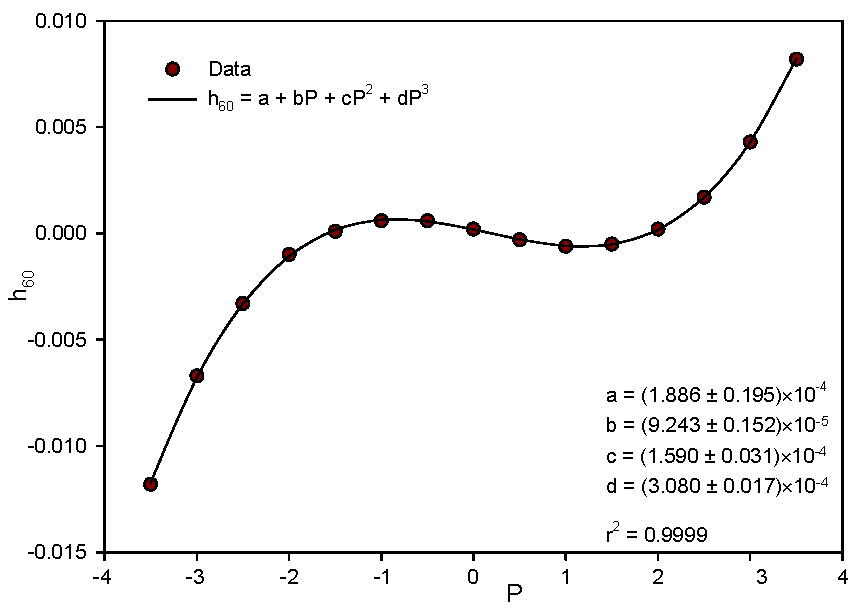
\includegraphics[width=0.75\textwidth]{Graphics/h60}
\end{figure}

Sometimes we have a desired probability for a given degree of freedom, and want to know how high the corresponding \skalar{\chi^2} needs to be. \parencite{Lia-68} gives three approximation, quadratic, cubic and improved cubic. Of these, the cubic is the most accurate for \( \nu \leq 10 \), and the improved cubic for \( \nu > 10 \):
\begin{equation}
  \chi^2(P|\nu) = \left\{
          \begin{array}{l@{\;}l}
             \nu \left[1 - \frac{2}{9 \nu}  + x_p \sqrt{\frac{2}{9 \nu}}\right]^3                           & \quad \forall \nu \leq 10  \\
             \nu \left[1 - \frac{2}{9 \nu} + (x_p - \frac{60 h(x_P)}{\nu}) \sqrt{\frac{2}{9 \nu}}\right]^3  & \quad \forall \nu > 10 \\
          \end{array}
        \right.
\end{equation}
The paper has a table of \skalar{h(x_P)}-values, but as can be seen in fig. \ref{fig:h60}, these can bee fitted very well with a polynom of 3rd order. \skalar{x_p} is such that the standardised normal probability function \( P(x_p) = 1 - P \).

\begin{lstlisting}[caption= \( \chi^2 \) required]
  FUNCTION SignificanceLimit_Chi2 (p : float; dgf : WORD) : float;

     FUNCTION H (x : float) : float;

     CONST a = 1.886e-4; b = 9.243e-5; c = 1.590e-4; d = 3.080e-4;

     BEGIN
       Result := a + b*x + c*x*x + d*x*x*x;
     END;

  VAR x, y : float;

  BEGIN
    y := -NormalStandardValue(p);
    IF dgf <= 10
      THEN x := (1 - 2/(9*dgf) + y                   * Sqrt(2/(9*dgf)))
      ELSE x := (1 - 2/(9*dgf) + (y - (h(y)*60/dgf)) * Sqrt(2/(9*dgf)));
    Result := dgf * x*x*x;
  END;
\end{lstlisting}

\subsection{The \skalar{G}-distribution}

The \skalar{G}-distribution \parencite{Sok-81} is related to the \skalar{\chi^2}-distribution and defined as
\begin{equation}
  G = 2 \sum_{i=1}^{n}{O_i \ln\left( \frac{O_i}{E_i} \right)}
\end{equation}
under the same conditions as for \skalar{\chi^2}. \skalar{G} follows a \skalar{\chi^2}-distribution with the same degrees of freedom, however, when used for small \skalar{n}, \skalar{G} approximates better than \Name{Pearson}'s \skalar{\chi^2}.

\section{\Name{Gauss}' normal distribution}

A continuous random variable \skalar{x \in \set{R}} is \Name{Gauss}ian normal distributed with mean \skalar{\mu} and variance \skalar{\sigma^2} (\( x \sim N(\mu, \sigma^2) \)), if \skalar{x} has the following probability density:
\begin{equation}
  f(x | \mu, \sigma^2) = \frac{1}{\sqrt{2\pi\sigma^2}} \exp\left( -\frac{(x-\mu)^2}{2\sigma^2} \right)
\end{equation}
This function has a bell-shaped, symmetrical  graph where \skalar{\mu} is the centre of symmetry and also the median and modus. \skalar{\mu\pm\sigma} are the inflexion points. The \textbf{standard normal distribution} has \( \mu = 0, \sigma^2 = 1\).

The integral of the \Name{Gauss}-distribution is:
\begin{equation}
  F(x | \mu, \sigma^2) = \frac{1}{\sqrt{2\pi}\sigma} \int_{-\infty}^{x} \exp\left[ -\frac{1}{2}\left(\frac{t-\mu}{\sigma}\right) \right] \mathrm{d}t
\end{equation}
Then for integration between
\begin{description}
  \item[ \( z1\ldots z2 \)]{\hspace{10mm}
     \begin{description}
        \item[\( z1 < 0 \) and \(z2 < 0 \)]{\( w = 0.5 * (\mathrm{GI}(\abs(z1)) - \mathrm{GI}(\abs(z2))) \)}
        \item[\( z1 > 0 \) and \(z2 > 0 \)]{\( w = 0.5 * (\mathrm{GI}(z1) + \mathrm{GI}(z2)) \)}
        \item[\( z1 < 0 \) and \(z2 > 0 \)]{\( w = 0.5 * (\mathrm{GI}(\abs(z1))) + \mathrm{GI}(z2) \)}
     \end{description}  }
  \item[\( -\infty\ldots z \)]{\hspace{10mm}
     \begin{description}
        \item[\( z > 0 \)]{\( w = 0.5 + 0.5 * \mathrm{GI}(z) \)}
        \item[\( z < 0 \)]{\( w = 0.5 - 0.5 * \mathrm{GI}(\abs(z)) \)}
     \end{description} }
  \item[ \( z\ldots \infty \)]{\hspace{10mm}
     \begin{description}
        \item[\( z > 0 \)]{\( w = 0.5 - 0.5 * \mathrm{GI}(z) \)}
        \item[\( z < 0 \)]{\( w = 0.5 + 0.5 * \mathrm{GI}(\abs(z)) \)}
     \end{description} }
\end{description}
The \textbf{central limit theorem} of \Name{Lindeberg \& Lévy} states, that the sum of (infinitely) many random variables is normally distributed, as long as none of the individual variables exerts a dominating influence on \skalar{\sigma}. Since  variables in nature are often determined by many interacting causes, the normal distribution is very common.

\begin{lstlisting}
  FUNCTION IntegralGauss(z: float): float;

  VAR
    f: float;


    FUNCTION Reihe(z: float): float;

    VAR
      Sum, G: float;
      i: INTEGER;

    BEGIN
      Sum := z;
      i := 1;
      G := z;
      REPEAT
        G := G * Sqr(z) / (2 * i + 1);
        INC(i);
        Sum := Sum + G;
      UNTIL G < MaxError;
      Result := Sum;
    END;

  BEGIN
    f := Exp(-Sqr(z) / 2) / Sqrt(2 * Pi);
    IntegralGauss := 2 * f * Reihe(z);
  END;
\end{lstlisting}

The next function calculates the factor with which the standard deviation needs to be multiplied so that any measured value is with a wanted probability in \(-nz\ldots +nz \):

\begin{lstlisting}[caption=]
  FUNCTION SignificanceLimitGauss(WantedSecurity: float): float;
  // -z ... z

  CONST
    a0 = 2.515517;    a1 = 0.802853;    a2 = 0.010328;
    b1 = 1.432788;    b2 = 0.189269;    b3 = 0.001308;

  VAR
    p, q, n, z0, f, p0, t: float;


    FUNCTION Reihe(z: float): float;

    VAR
      Sum, G: float;
      i: INTEGER;

    BEGIN
      Sum := z;
      i := 1;
      G := z;
      REPEAT
        G := G * Sqr(z) / (2 * i + 1);
        INC(i);
        Sum := Sum + G;
      UNTIL G < MaxError;
      Result := Sum;
    END;

  BEGIN
    q := (1 - WantedSecurity) / 2;
    p := 1 - q;
    n := Sqrt(Ln(1 / Sqr(q)));
    z0 := n - (a0 + n * (a1 + a2 * n)) / (1 + n * (b1 + n * (b2 + b3 * n)));
    f := Exp(-Sqr(z0) / 2) / Sqrt(2 * Pi);
    p0 := 0.5 + f * Reihe(z0);
    t := (p - p0) / f;
    Result := z0 + t + z0 * Sqr(t) / 2 + (2 * Sqr(z0) + 1) / 6 * pot(t, 3);
  END;
\end{lstlisting}


The next function calculates the factor with which the standard deviation needs to be multiplied so that any measured value is with a wanted probability in \(-\infty\ldots +nz \). It is based on \parencite{Vou-10}.

\begin{lstlisting}[caption=Normal standard value]
  FUNCTION NormalStandardValue (P : float) : float;

  CONST a0 = 0.389422403767615;     a1 = -1.699385796345221; a2 = 1.246899760652504;
        b0 = 0.155331081623168;     b1 = -0.839293158122257;
        c0 = 16.896201479841517652; c1 = -2.793522347562718412;
        c2 = -8.731478129786263127; c3 = -1.000182518730158122;
        d0 = 7.173787663925508066;  d1 = 8.759693508958633869;

  VAR q, r : float;
      c    : CHAR;

  BEGIN
    IF (P < 1e-298) OR (P > (1-1e-298))
      THEN
        BEGIN
          c := WriteErrorMessage('Normal standard value: Value outside range');
          Result := NaN;
          StatError := TRUE;
          EXIT;
        END;
    IF P < 0.0465
      THEN  // lower tail
        BEGIN
          r := Sqrt(Ln(1/(P*P)));
          Result := (c0 + c1*r + c2*r*r + c3*r*r*r) / (d0 + d1*r + r*r);
        END
      ELSE
        IF P < 0.9535
          THEN  // central region
            BEGIN
              q := p-0.5;
              r := q*q;
              Result := q * (a0 + a1*r + a2*r*r) / (b0 + b1*r + r*r);
            END
          ELSE  // upper tail
            BEGIN
              q := 1-p;
              r := Sqrt(Ln(1/(q*q)));
              Result := -(c0 + c1*r + c2*r*r + c3*r*r*r) / (d0 + d1*r + r*r);
            END;
  END;
\end{lstlisting}

The \Name{Gauss}ian error function is
\begin{equation}
   \mathrm{erf}(x) = \frac{2}{\sqrt{\pi}} \int_{0}^{x} \mathrm{e}^{-r^2} \mathrm{d}r \approx \frac{2}{\sqrt{\pi}} \sum_{n=0}^{\infty} \frac{(-1)^n x^{2n + 1}}{(2n + 1) n!}
 \end{equation}
, which for \( x \in \set{R} \) returns real numbers in \( [-1\ldots +1] \). The generalisation to complex arguments is of no interest here. The conjugated error function is
\begin{equation}
  \mathrm{erfc} (x) = \frac{2}{\sqrt{\pi}} \int_{x}^{\infty} \mathrm{e}^{-r^2} \mathrm{d}r = 1 - \mathrm{erf}(x)
\end{equation}

\begin{lstlisting}[caption=Error function]
  FUNCTION Erf (Z : float) : float;

  CONST A:  ARRAY[1..14] OF float =
            ( 1.1283791670955,       0.34197505591854,     0.86290601455206E-1,
              0.12382023274723E-1,   0.11986242418302E-2,  0.76537302607825E-4,
              0.25365482058342E-5,  -0.99999707603738,    -1.4731794832805,
             -1.0573449601594,      -0.44078839213875,    -0.10684197950781,
             -0.12636031836273E-1,  -0.1149393366616E-8  );

        B:  ARRAY[1..12] OF REAL =
            ( -0.36359916427762,     0.52205830591727E-1, -0.30613035688519E-2,
              -0.46856639020338E-4,  0.15601995561434E-4, -0.62143556409287E-6,
               2.6015349994799,      2.9929556755308,      1.9684584582884,
               0.79250795276064,     0.18937020051337,     0.22396882835053E-1 );

  VAR U, X, S:  float;

  BEGIN
    X := ABS(Z);                 (* Get absolute value of argument *)
    S := Signum(Z);              (* Remember sign of argument *)
    IF ( S = 0.0 )               (* Check for zero argument *)
      THEN
        Result := 0.0
      ELSE                       (* Check for large argument *)
        IF (X >= 5.5)
          THEN
            Result := S
          ELSE                   (* Arg in approximation range *)
            BEGIN
                U := X * X;
                IF (X <= 1.5)
                  THEN           (* Approx. for arg <= 1.5 *)
                    Result := (X * EXP(-U) * (A[1] + U * (A[2] + U *
                              (A[3] + U * (A[4] + U * (A[5] + U *
                              (A[6] + U * A[7] )))))) /
                              (1.0 + U * (B[1] + U * (B[2] + U *
                              (B[3] + U * (B[4] + U * (B[5] + U *
                              B[6] ))))))) * S
                  ELSE          (* Approx. for arg > 1.5 *)
                    Result := (EXP(-U) * (A[8] + X * (A[9] + X * (A[10] + X *
                              (A[11] + X * (A[12] + X * (A[13] + X * A[14] )))))) /
                              (1.0 + X * (B[7] + X * (B[8] + X * (B[9] + X *
                              (B[10] + X * (B[11] + X * B[12])))))) + 1.0) * S;
            END;
  END;   (* Erf *)
\end{lstlisting}

The error function is related to the normal distribution with standard deviation \skalar{\sigma} and expected value \skalar{\mu}
\begin{equation}
  F(x) = \frac{1}{2} \left[ 1 + \mathrm{erf}\left( \frac{x-\mu}{\sigma \sqrt{2}} \right) \right]
\end{equation}

\begin{lstlisting}[caption=Tail probability of normal distribution]
  FUNCTION SigNorm (X : float) : float;

  BEGIN
      IF X >= 0.0
        THEN Result := 1.0 - (1.0 + Erf(X / Const_Sqrt2)) / 2.0
        ELSE Result := 1.0 - (1.0 - Erf(-X / Const_Sqrt2)) / 2.0;
  END   (* SigNorm *);
\end{lstlisting}

\begin{lstlisting}[caption=Cumulative normal distribution probability]
  FUNCTION CDNorm (X : float) : float;

  BEGIN
     IF X >= 0.0
       THEN Result := ( 1.0 + Erf(  X / Const_Sqrt2 ) ) / 2.0
       ELSE Result := ( 1.0 - Erf( -X / Const_Sqrt2 ) ) / 2.0;
  END;
\end{lstlisting}

An alternative way to calculate the percentage point of the normal distribution with about \num{6} valid figures is
\begin{lstlisting}[caption=percentage point of normal distribution]
  FUNCTION NinvCoarse (P : float) : float;

  CONST Lim = 1.0E-20;

  VAR Y :  float;
      Pr: float;
      Nv: float;

  CONST PN : ARRAY [1..5] OF float =
             ( -0.322232431088  ,  -1.0              , -0.342242088547  ,
               -0.0204231210245 ,  -0.453642210148E-4 );

         QN : ARRAY [1..5] OF float =
             ( 0.0993484626060 ,    0.588581570495   ,  0.531103462366  ,
               0.103537752850  ,    0.38560700634E-2  );

  BEGIN (* NinvCoarse *)
    Result := 0.0;
    IF (P > 0.5)
      THEN Pr := 1.0 - P
      ELSE Pr := P;
    IF (( Pr >= Lim ) AND ( Pr <> 0.5 ))
      THEN
        BEGIN
          Y := SQRT ( LN( 1.0 / Pr / Pr ) );
          Nv := Y + ((((Y * PN[ 5 ] + PN[ 4 ]) * Y + PN[ 3 ] ) * Y
                                    + PN[ 2 ]) * Y + PN[ 1 ] ) /
                    ((((Y * QN[ 5 ] + QN[ 4 ]) * Y + QN[ 3 ] ) * Y
                                    + QN[ 2 ]) * Y + QN[ 1 ] );
          IF (P < 0.5)
            THEN Result := -Nv
           ELSE Result := Nv;
        END;
  END   (* NinvCoarse *);
\end{lstlisting}
This result can be made precise to \num{12} valid figures by using a \Name{Taylor} series on the approximation error:
\begin{lstlisting}[caption=percentage point of normal distribution]
  FUNCTION Ninv( P : float ) : float;

  VAR Xp, P1, Z, X3, X2, X1, Phi: float;

  BEGIN
    Xp := Ninv(P);
    P1 := SigNorm(Xp);
    Phi := SQRT(1.0 / (2.0 * PI)) * EXP(-(Xp * Xp) / 2.0);
    Z  := (P - P1) / Phi;
    X3 := (2.0 * (Xp * Xp) + 1.0) * Z / 3.0;
    X2 := (X3 + Xp) * Z / 2.0;
    X1 := ((X2 + 1.0) * Z);
    Result := Xp + X1;
  END   (* Ninv *);
\end{lstlisting}


\section{Binomial distribution}

The binomial frequency is the probability to have \texttt{Success} successes out of \texttt{trials} attempts, when the success probability per attempt is \skalar{P}

\begin{lstlisting}[caption=Routines for the binomial distribution]
  FUNCTION BinominalFrequency(Trials, Success: LONGINT; P: float): float;

  VAR
    TrialsOverSuccess: float;

  BEGIN
    TrialsOverSuccess := BinomialCoef(Trials, Success);
    Result := TrialsOverSuccess * pot(P, Success) *
      pot(1 - P, Trials - Success);
  END;
\end{lstlisting}

The integral is the probability that the number of successes is less or equal than \texttt{Value}, when the number of trials is \texttt{Trials} and the probability of success in each trial is \skalar{P}.

\begin{lstlisting}[caption=]
  FUNCTION BinominalIntegral(Trials, Value: LONGINT; P: float): float;

  VAR
    Sum: float;
    i: WORD;

  BEGIN
    Sum := 0.0;
    FOR i := 0 TO Value DO
      Sum := Sum + BinominalFrequency(Trials, i, P);
    Result := Sum;
  END;
\end{lstlisting}

\section{The \Name{Pareto} (80/20) distribution}

The \Name{Pareto} distribution \parencite{Par-87} describes a continuous function on the interval \([x_\mathrm{min}, \infty]\), the cumulative distribution function of the \Name{Pareto}-distribution with Minimum \(x_\mathrm{min} \geq 0 \), Shape \(k > 1 \) is
\begin{equation}
  f(x) = \left\{
     \begin{array}{lr}
         \frac{k x_\mathrm{min}^k}{x^{k+1}} & x \geq x_\mathrm{min} \\
         0                                  & x < x_\mathrm{min}
     \end{array}
  \right.
\end{equation}
This distribution can describe parameters that cover several orders of magnitude and depend on many random factors. The \Name{Pareto}-principle says that the lowest \SI{20}{\%} of the independent variable account for \SI{80}{\%} of the dependent variable (law of diminishing return), then \(k \approx\ 1.16\).


\begin{lstlisting}[caption=The \Name{Pareto} distribution]
  FUNCTION IntegralPareto(x, Minimum, Shape: float): float;

  BEGIN
    Result := 1 - Pot((Minimum / x), Shape);
  END;


  FUNCTION ProbabilityDistributionFunctionPareto(x, Minimum, Shape: float): float;

  BEGIN
    Result := Shape * pot(Minimum, Shape) / pot(x, Shape + 1);
  END;


  END.  // Stat
\end{lstlisting}

\section{The \textbeta-distribution}

\begin{lstlisting}[caption=\textbeta distribution]
  FUNCTION CDBeta (X, Alpha, Beta : float; Dprec, MaxIter : INTEGER;
                   VAR Cprec      : float; VAR Iter       : INTEGER;
                   VAR Ifault     : INTEGER  ) : float;

  VAR Epsz, A, B, C,
      F, Fx, Apb, Zm,
      Alo, Ahi, Aev, Aod,
      Blo, Bhi, Bod, Bev,
      Zm1, D1             : float;
      Ntries              : INTEGER;
      Qswap, Qdoit, Qconv : BOOLEAN;

  LABEL   20;

  BEGIN
    (* Initialize *)
    IF Dprec > MaxPrec
      THEN Dprec := MaxPrec
      ELSE IF Dprec <= 0
             THEN Dprec := 1;
    Cprec := Dprec;
    Epsz := pot(10, -Dprec);
    X := X;
    A := Alpha;
    B := Beta;
    QSwap  := FALSE;
    CDBeta := -1.0;
    Qdoit  := TRUE;
    (* Check arguments. Error if: X <= 0  or  A <= 0  or  B <= 0       *)
    Ifault := 1;
    IF (X <= 0.0) or ((A <= 0.0) OR (B <= 0.0)) OR ( X >= 1.0 )
      THEN
        BEGIN
          ch := WriteErrorMessage('CDBeta: illegal arguments');
          StatError := TRUE;
          EXIT;
        END;
    CDBeta := 1.0;
    Ifault := 0;
    (* If X > A / ( A + B ) then swap A, B for more efficient eval.  *)
    IF (X > (A / (A + B)))
      THEN
        BEGIN
          X      := 1.0 - X;
          A      := Beta;
          B      := Alpha;
          QSwap  := TRUE;
        END;
    (* Check for extreme values *)
    IF ((X = A) OR (X = B)) THEN GOTO 20;
    IF (A = ((B * X) / (1.0 - X))) THEN GOTO 20;
    IF (ABS(A - (X * (A + B))) <= Epsz ) THEN GOTO 20;
    C := ALGama(A + B) + A * LN(X) + B * LN(1.0 - X) - ALGama(A) -
         ALGama(B) - LN(A - X * (A + B));
    IF ((C < -36.0) AND QSwap) OR (C < -180.0)
      THEN
        BEGIN
          ch := WriteErrorMessage('CDBeta: extreme values outside computable range');
          StatError := TRUE;
          EXIT;
        END;
    CDBeta := 0.0;
    (*  Set up continued fraction expansion evaluation. *)
    20:
    Apb := A + B;
    Zm  := 0.0;
    Alo := 0.0;
    Bod := 1.0;
    Bev := 1.0;
    Bhi := 1.0;
    Blo := 1.0;
    Ahi := EXP(ALGama(Apb) + A * LN(X) + B * LN(1.0 - X) -
           ALGama(A + 1.0) - ALGama(B));
    F   := Ahi;
    Iter := 0;
    (* Continued fraction loop begins here. Evaluation continues until
    maximum iterations are exceeded, or convergence achieved.       *)
    Qconv  := FALSE;
    REPEAT
      Fx  := F;
      Zm1 := Zm;
      Zm  := Zm + 1.0;
      D1  := A + Zm + Zm1;
      Aev := -( A + Zm1 ) * ( Apb + Zm1 ) * X / D1 / ( D1 - 1.0 );
      Aod := Zm * ( B - Zm ) * X / D1 / ( D1 + 1.0 );
      Alo := Bev * Ahi + Aev * Alo;
      Blo := Bev * Bhi + Aev * Blo;
      Ahi := Bod * Alo + Aod * Ahi;
      Bhi := Bod * Blo + Aod * Bhi;
      IF ABS (Bhi) < MinRealNumber THEN Bhi := 0.0;
      IF (Bhi <> 0.0)
        THEN
          BEGIN
            F     := Ahi / Bhi;
            Qconv := (ABS((F - Fx) / F) < Epsz);
          END;
      Iter  := Iter + 1;
    UNTIL ( ( Iter > MaxIter ) OR Qconv ) ;
    (* Arrive here when convergence achieved, or maximum iterations exceeded.  *)
    IF (Qswap)
      THEN CDBeta := 1.0 - F
      ELSE CDBeta := F;
    (* Calculate precision of result *)
    IF ABS(F - Fx) <> 0.0
      THEN Cprec := -Log(ABS(F - Fx), 10)
      ELSE Cprec := MaxPrec;
  END;   (* CDBeta *)


  FUNCTION BetaInv (P, Alpha, Beta : float; MaxIter, Dprec: INTEGER;
                    VAR Iter : INTEGER; VAR Cprec : float; VAR Ierr: INTEGER) : float;

  VAR Eps, Xim1, Xi, Xip1, Fim1, Fi,
      W, Cmplbt, Adj, Sq, R, S, T,
      G, A, B, PP, H, A1, B1, Eprec  : float;
      Done                           : BOOLEAN;
      Jter                           : INTEGER;

  LABEL 10, 30;

  BEGIN
    Ierr    := 1;
    Result := P;
  (* Check validity of arguments *)
    IF ((Alpha <= 0.0) OR (Beta <= 0.0)) OR  ((P > 1.0) OR (P < 0.0))
      THEN
        BEGIN
          ch := WriteErrorMessage('BetaInv: illegal parameters');
          StatError := TRUE;
          Result := -1.0;
          EXIT;
        END;
  (* Check for P = 0 or 1        *)
    IF ((P = 0.0) OR (P = 1.0))
      THEN
        BEGIN
          Iter   := 0;
          Cprec  := MaxPrec;
          EXIT;
        END;
  (* Set precision *)
    IF Dprec > MaxPrec
      THEN Dprec := MaxPrec
      ELSE IF Dprec <= 0
             THEN Dprec := 1;
    Cprec  := Dprec;
    Eps    := pot(10, -2 * Dprec);
  (* Flip params if needed so that P for evaluation is <= .5     *)
    IF (P > 0.5)
      THEN
        BEGIN
          A  := Beta;
          B  := Alpha;
          PP := 1.0 - P;
        END
      ELSE
        BEGIN
          A  := Alpha;
          B  := Beta;
          PP := P;
        END;
  (* Generate initial approximation. Several different ones used, depending upon parameter values. *)
    Ierr   := 0;
    Cmplbt := ALGama(A) + ALGama(B) - ALGama(A + B);
    Fi     := Ninv(1.0 - PP);
    IF ((A > 1.0) AND (B > 1.0))
      THEN
        BEGIN
          R := (Fi * Fi - 3.0) / 6.0;
          S := 1.0 / (A + A - 1.0);
          T := 1.0 / (B + B - 1.0);
          H := 2.0 / (S + T);
          W := Fi * SQRT(H + R) / H - (T - S) * (R + 5.0 / 6.0 - 2.0 / (3.0 * H));
          Xi:= A / (A + B * EXP(W + W));
         END
       ELSE
         BEGIN
           R := B + B;
           T := 1.0 / (9.0 * B);
           T := R * Pot((1.0 - T + Fi * SQRT(T)), 3);
           IF (T <= 0.0)
             THEN
               Xi := 1.0 - EXP((LN((1.0 - PP) * B) + Cmplbt) / B)
             ELSE
               BEGIN
                 T      := ( 4.0 * A + R - 2.0 ) / T;
                 IF (T <= 1.0)
                   THEN Xi := EXP((LN(PP * A) + Cmplbt) / PP)
                   ELSE Xi := 1.0 - 2.0 / (T + 1.0);
               END;
         END;
  (* Force initial estimate to reasonable range.         *)
    IF (Xi < 0.0001) THEN Xi := 0.0001;
    IF (Xi > 0.9999) THEN Xi := 0.9999;
  (* Set up Newton-Raphson loop *)
    A1   := 1.0 - A;
    B1   := 1.0 - B;
    Fim1 := 0.0;
    Sq   := 1.0;
    Xim1 := 1.0;
    Iter := 0;
    Done := FALSE;
  (* Begin Newton-Raphson loop  *)
    REPEAT
      Iter := Iter + 1;
      Done := Done OR (Iter > MaxIter);
      Fi   := CDBeta(Xi, A, B, Dprec+1, MaxIter, Eprec, Jter, Ierr);
      IF (Ierr <> 0)
       THEN
         BEGIN
           Ierr := 2;
           Done := TRUE;
         END
       ELSE
         BEGIN
           Fi := (Fi - PP) * EXP(Cmplbt + A1 * LN(Xi) + B1 * LN(1.0 - Xi));
           IF ((Fi * Fim1) <= 0.0) THEN Xim1 := Sq;
           G := 1.0;
  10:      REPEAT
             Adj := G * Fi;
             Sq  := Adj * Adj;
             IF (Sq >= Xim1) THEN G := G / 3.0;
           UNTIL (Sq < Xim1);
           Xip1 := Xi - Adj;
           IF ((Xip1 < 0.0) OR (Xip1 > 1.0))
             THEN
               BEGIN
                 G := G / 3.0;
                 GOTO 10;
               END;
           IF (Xim1 <= Eps) THEN GOTO 30;
           IF (Fi * Fi <= Eps) THEN GOTO 30;
           IF ((Xip1 = 0.0) OR (Xip1 = 1.0))
             THEN
               BEGIN
                 G := G / 3.0;
                 GOTO 10;
               END;
           IF (Xip1 <> Xi)
             THEN
               BEGIN
                 Xi := Xip1;
                 Fim1 := Fi;
               END
             ELSE
               Done := TRUE;
         End;
    UNTIL( Done );
  30:
    Result := Xi;
    IF (P > 0.5) THEN Result := 1.0 - Xi;
    IF ABS(Xi - Xim1) <> 0.0
      THEN
         Cprec := -log(ABS(Xi - Xim1), 10)
      ELSE
         Cprec  := MaxPrec;
  END   (* BetaInv *);
\end{lstlisting}


\section{The \textGamma-distribution}

\Name{Euler}'s \textGamma-function for \( n \in \set{N} \) is
\begin{equation}
  \Gamma(n) = (n-1)! = \int_{0}^{\infty} t^{n-1} \mathrm{e}^{-t} \mathrm{d}t
\end{equation}
with \( t = -\log(n) \). This function can be expanded to \set{R} and \set{C}:
\begin{equation}
  \Gamma(x) = \lim_{n\rightarrow\infty} \frac{n!n^x}{x(x+1)(x+2)\ldots (x+n)} = \int_{0}^{\infty} t^{x-1} \mathrm{e}^{-t} dt\quad \forall\quad \mathrm{Re}(x) > 0
\end{equation}
The upper incomplete \textgamma-function is
\begin{equation}
  \gamma(a, x) = \int_{0}^{x} t^{a-1} \mathrm{e}^{-t} \mathrm{d}t
\end{equation}
, for the lower incomplete \textgamma-function the integration limits are \skalar{x} and \skalar{\infty}.

The \textGamma-distribution \skalar{G(x | \beta, \alpha)} has the density and distribution function
\begin{eqnarray}
  f(x) &=& \left\{
             \begin{array}{lr}
                \frac{b^\alpha}{\Gamma(\alpha)} x^{\alpha-1} \mathrm{e}^{-\beta x} & x > 0 \\
                0                                                                  & x \leq 0
             \end{array}
           \right.  \\
  F(x) &=& \left\{
              \begin{array}{lr}
                 \gamma(\alpha, \beta x)  & x \geq 0  \\
                 0                        & x < 0
              \end{array}
           \right.
\end{eqnarray}
with the inverse scale parameter \skalar{\beta > 0} and the shape parameter \skalar{\alpha > 0}.

\begin{lstlisting}[caption=\textgamma distribution]
  FUNCTION ALGama( Arg : float ) : float;

  VAR
     Rarg, Alinc, Scale, Top, Bot, Frac, Algval : float;
     I, Iapprox, Iof, Ilo, Ihi                  : INTEGER;
     Qminus, Qdoit                              : BOOLEAN;


  CONST P : ARRAY [1..29] OF float =
                   ( 4.12084318584770E+00 ,  8.56898206283132E+01 ,
                     2.43175243524421E+02 , -2.61721858385614E+02 ,
                    -9.22261372880152E+02 , -5.17638349802321E+02 ,
                    -7.74106407133295E+01 , -2.20884399721618E+00 ,
                     5.15505761764082E+00 ,  3.77510679797217E+02 ,
                     5.26898325591498E+03 ,  1.95536055406304E+04 ,
                     1.20431738098716E+04 , -2.06482942053253E+04 ,
                    -1.50863022876672E+04 , -1.51383183411507E+03 ,
                    -1.03770165173298E+04 , -9.82710228142049E+05 ,
                    -1.97183011586092E+07 , -8.73167543823839E+07 ,
                     1.11938535429986E+08 ,  4.81807710277363E+08 ,
                    -2.44832176903288E+08 , -2.40798698017337E+08 ,
                     8.06588089900001E-04 , -5.94997310888900E-04 ,
                     7.93650067542790E-04 , -2.77777777688189E-03 ,
                     8.33333333333330E-02   );

     Q : ARRAY [1..24] OF float =
                   ( 1.00000000000000E+00 ,  4.56467718758591E+01 ,
                     3.77837248482394E+02 ,  9.51323597679706E+02 ,
                     8.46075536202078E+02 ,  2.62308347026946E+02 ,
                     2.44351966250631E+01 ,  4.09779292109262E-01 ,
                     1.00000000000000E+00 ,  1.28909318901296E+02 ,
                     3.03990304143943E+03 ,  2.20295621441566E+04 ,
                     5.71202553960250E+04 ,  5.26228638384119E+04 ,
                     1.44020903717009E+04 ,  6.98327414057351E+02 ,
                     1.00000000000000E+00 , -2.01527519550048E+03 ,
                    -3.11406284734067E+05 , -1.04857758304994E+07 ,
                    -1.11925411626332E+08 , -4.04435928291436E+08 ,
                    -4.35370714804374E+08 , -7.90261111418763E+07   );

  BEGIN
    Algval := MaxRealNumber;   // Initialize
    Scale  := 1.0;
    Alinc  := 0.0;
    Frac   := 0.0;
    Rarg   := Arg;
    Iof    := 1;
    Qminus := FALSE;
    Qdoit  := TRUE;
    IF (Rarg < 0.0)           // Adjust for negative argument
      THEN
        BEGIN
          Qminus := TRUE;
          Rarg   := -Rarg;
          Top    := Int( Rarg );
          Bot    := 1.0;
          IF((INT(Top / 2.0) * 2.0) = 0.0) THEN Bot := -1.0;
          Top    := Rarg - Top;
          IF (Top = 0.0)
            THEN
              Qdoit := FALSE
            ELSE
              BEGIN
                Frac   := Bot * CONST_PI / SIN( Top * CONST_PI );
                Rarg   := Rarg + 1.0;
                Frac   := LN( ABS( Frac ) );
              END;
        END;
  { Choose approximation interval based upon argument range }
    IF (Rarg = 0.0)
      THEN
        Qdoit := FALSE
      ELSE
        IF (Rarg <= 0.5)
          THEN
            BEGIN
              Alinc  := -LN( Rarg );
              Scale  := Rarg;
              Rarg   := Rarg + 1.0;
              IF (Scale < MachineEpsilon)
                THEN
                  BEGIN
                    Algval := Alinc;
                    Qdoit  := FALSE;
                  END;
            END
          ELSE
            IF (Rarg <= 1.5)
              THEN
                Scale := Rarg - 1.0
              ELSE
                IF (Rarg <= 4.0)
                  THEN
                    BEGIN
                      Scale  := Rarg - 2.0;
                      Iof    := 9;
                    END
                  ELSE
                    IF (Rarg <= 12.0)
                     THEN
                       Iof := 17
                     ELSE
                       IF (Rarg <= MaxRealNumber)
                         THEN
                           BEGIN
                             Alinc  := ( Rarg - 0.5 ) * LN( Rarg ) - Rarg + Xln2sp;
                             Scale  := 1.0 / Rarg;
                             Rarg   := Scale * Scale;
                             Top    := P[ 25 ];
                             for i := 26 to 29 do Top := Top * Rarg + P[ I ];
                             Algval := Scale * Top + Alinc;
                             Qdoit  := FALSE;
                           END;
  { Common evaluation code for Arg <= 12. Horner's method is used, which seems to
  give better accuracy than continued fractions. }
    IF Qdoit
      THEN
        BEGIN
          Ilo    := Iof + 1;
          Ihi    := Iof + 7;
          Top    := P[ Iof ];
          Bot    := Q[ Iof ];
          FOR I := Ilo TO Ihi DO
             BEGIN
                 Top    := Top * Rarg + P[ I ];
                 Bot    := Bot * Rarg + Q[ I ];
             END;
          Algval := Scale * ( Top / Bot ) + Alinc;
        END;
     IF (Qminus) THEN Algval := Frac - Algval;
     Result := Algval;
  END;   (* ALGama *)


  FUNCTION GammaInt (Y, P : float; Dprec, MaxIter : INTEGER;
                    VAR Cprec : float; VAR Iter, Ifault  : INTEGER ) : float;

  CONST Oflo    = 1.0E+37;
        MinExp  = -87.0;

  VAR F, C, A, B,Term, An, Gin, Rn, Dif, Eps : float;
     Pn                                      : ARRAY[1..6] OF float;
     Done                                    : BOOLEAN;

  BEGIN
  (* Check arguments *)
    Ifault  := 1;
    Result := 1.0;
    IF ((Y <= 0.0) OR (P <= 0.0))
      THEN
        BEGIN
          ch := WriteErrorMessage('Gamma integralv: illegal parameters');
          StatError := TRUE;
          EXIT;
       END;
  (* Check value of F *)
    Ifault := 0;
    F := P * LN(Y) - ALGama(P + 1.0) - Y;
    IF (F < MinExp)
      THEN
        BEGIN
          ch := WriteErrorMessage('Gamma integralv: extreme value not computable');
          StatError := TRUE;
          EXIT;
       END;
    F := EXP(F);
    IF (F = 0.0)
      THEN
        BEGIN
          ch := WriteErrorMessage('Gamma integralv: extreme value not computable');
          StatError := TRUE;
          EXIT;
       END;
  (* Set precision *)
    IF Dprec > MaxPrec
      THEN Dprec := MaxPrec
      ELSE IF Dprec <= 0 THEN Dprec := 1;
    Cprec := Dprec;
    Eps := Pot(10, -Dprec);
  (* Choose infinite series or continued fraction.       *)
    IF ((Y > 1.0) AND (Y >= P))
      THEN
        BEGIN (* Continued Fraction *)
          A := 1.0 - P;
          B := A + Y + 1.0;
          Term := 0.0;
          Pn[1] := 1.0;
          Pn[2] := Y;
          Pn[3] := Y + 1.0;
          Pn[4] := Y * B;
          Gin := Pn[3] / Pn[4];
          Done := FALSE;
          Iter := 0;
          REPEAT
            Iter := Iter + 1;
            A := A + 1.0;
            B := B + 2.0;
            Term := Term + 1.0;
            An := A * Term;
            Pn[5] := B * Pn[3] - An * Pn[1];
            Pn[6] := B * Pn[4] - An * Pn[2];
            IF (Pn[6] <> 0.0)
              THEN
                 BEGIN
                     Rn := Pn[ 5 ] / Pn[ 6 ];
                     Dif := ABS(Gin - Rn);
                     IF (Dif <= Eps)
                       THEN
                          IF (Dif <= (Eps * Rn)) THEN Done := TRUE;
                     Gin := Rn;
                 END;
            Pn[1] := Pn[3];
            Pn[2] := Pn[4];
            Pn[3] := Pn[5];
            Pn[4] := Pn[6];
            IF (ABS(Pn[5]) >= Oflo)
              THEN
                BEGIN
                  Pn[1] := Pn[1] / Oflo;
                  Pn[2] := Pn[2] / Oflo;
                  Pn[3] := Pn[3] / Oflo;
                  Pn[4] := Pn[4] / Oflo;
                END;
          UNTIL (Iter > MaxIter) OR Done;
          Gin := 1.0 - (F * Gin * P);
          Result := Gin;
  (* Calculate precision of result *)
          IF Dif <> 0.0
            THEN Cprec := -Log(Dif, 10)
            ELSE Cprec := MaxPrec;
        END   (* Continued Fraction *)
      ELSE
        BEGIN (* Infinite series *)
          Iter := 0;
          Term := 1.0;
          C := 1.0;
          A := P;
          Done := FALSE;
          REPEAT
            A := A + 1.0;
            Term := Term * Y / A;
            C := C + Term;
            Iter := Iter + 1;
          UNTIL (Iter > MaxIter) OR ((Term / C) <= Eps);
          Result := C * F;
  (* Calculate precision of result *)
          Cprec := -Log(Term / C, 10);
        END   (* Infinite series *);
  END;    (* GammaIn *)
\end{lstlisting}

\section{\Name{Kolmogorov-Smirnov}-test}

The \Name{Kolmogorov-Smirnov}-test is used to test \textbf{H\textsubscript{0}: Two random variables have the same distribution (\( F_1(x) = F_2(x) \))} against \textbf{H\textsubscript{1}: The two random variables have different distributions (\( F_1(x) \neq F_2(x) \))}. The second variable can be either experimental (two sample test), or can come from a theoretical distribution (one sample test). This can be used, for example, to test whether a sample is normally distributed; and therefore, whether tests relying on this distribution are applicable.

For the test, both samples are sorted in ascending order. Then \( d_n = ||F_1 - F_2|| = \mathrm{sup}|F_1(x) - F_2(x)| \), where the supremum of a set is defined as the smallest number that is larger than all members of the set. For example, for the set of real numbers \(< 2\), two is the supremum: the set contains no number larger than \skalar {2}, and no number smaller than \num{2} is larger than all members of the set.

In other words, the cumulative distribution of both functions are plotted, and \skalar{d_n} is the largest distance between both curves. Since the test is non-parametric, it works better for small samples than the \skalar{\chi^2}-test, and it works independent of the actual distribution of the variables. It was developed for continuous variables, but also works for discrete or rank-scaled variables. It is, however, less sensitive than parametric tests would be. 

The following routine calculates the probability for the 0-hypothesis in the \Name{Kolmogorov-Smirnov}-test. \texttt{alam} is
\begin{itemize}
  \item{\( d \sqrt{n} \) for the 1-sample test}
  \item{\( d \sqrt{\frac{n_1*n_2}{(n_1+n_2)}} \) for the 2-sample test}
\end{itemize}

\begin{lstlisting}[caption=\Name{Kolmogorov-Smirnov}-test]
  FUNCTION KolmogorovSmirnovIntegral(alam: float): float;

  CONST
    eps1 = 0.001;
    eps2 = 1.0e-8;

  VAR
    a2, fac, sum, term, termbf: float;
    j: INTEGER;

  BEGIN
    a2 := -2.0 * alam * alam;
    fac := 2.0;
    sum := 0.0;
    termbf := 0.0;
    FOR j := 1 TO 100 DO
      BEGIN
        term := fac * Exp(a2 * Sqr(j));
        sum := sum + term;
        IF ((Abs(term) < (eps1 * termbf)) OR (Abs(term) < (eps2 * sum)))
          THEN
            BEGIN     // convergence reached
              Result := sum;
              EXIT;
            END
          ELSE
            BEGIN
              fac := -fac;
              termbf := Abs(term);
            END;
      END;
    Result := 1.0;
  END;
\end{lstlisting}

\printbibliography[heading=subbibliography]
\end{refsection}

